% Options for packages loaded elsewhere
\PassOptionsToPackage{unicode}{hyperref}
\PassOptionsToPackage{hyphens}{url}
%
\documentclass[
]{article}
\usepackage{amsmath,amssymb}
\usepackage{lmodern}
\usepackage{iftex}
\ifPDFTeX
  \usepackage[T1]{fontenc}
  \usepackage[utf8]{inputenc}
  \usepackage{textcomp} % provide euro and other symbols
\else % if luatex or xetex
  \usepackage{unicode-math}
  \defaultfontfeatures{Scale=MatchLowercase}
  \defaultfontfeatures[\rmfamily]{Ligatures=TeX,Scale=1}
\fi
% Use upquote if available, for straight quotes in verbatim environments
\IfFileExists{upquote.sty}{\usepackage{upquote}}{}
\IfFileExists{microtype.sty}{% use microtype if available
  \usepackage[]{microtype}
  \UseMicrotypeSet[protrusion]{basicmath} % disable protrusion for tt fonts
}{}
\makeatletter
\@ifundefined{KOMAClassName}{% if non-KOMA class
  \IfFileExists{parskip.sty}{%
    \usepackage{parskip}
  }{% else
    \setlength{\parindent}{0pt}
    \setlength{\parskip}{6pt plus 2pt minus 1pt}}
}{% if KOMA class
  \KOMAoptions{parskip=half}}
\makeatother
\usepackage{xcolor}
\usepackage[margin=1in]{geometry}
\usepackage{color}
\usepackage{fancyvrb}
\newcommand{\VerbBar}{|}
\newcommand{\VERB}{\Verb[commandchars=\\\{\}]}
\DefineVerbatimEnvironment{Highlighting}{Verbatim}{commandchars=\\\{\}}
% Add ',fontsize=\small' for more characters per line
\usepackage{framed}
\definecolor{shadecolor}{RGB}{248,248,248}
\newenvironment{Shaded}{\begin{snugshade}}{\end{snugshade}}
\newcommand{\AlertTok}[1]{\textcolor[rgb]{0.94,0.16,0.16}{#1}}
\newcommand{\AnnotationTok}[1]{\textcolor[rgb]{0.56,0.35,0.01}{\textbf{\textit{#1}}}}
\newcommand{\AttributeTok}[1]{\textcolor[rgb]{0.77,0.63,0.00}{#1}}
\newcommand{\BaseNTok}[1]{\textcolor[rgb]{0.00,0.00,0.81}{#1}}
\newcommand{\BuiltInTok}[1]{#1}
\newcommand{\CharTok}[1]{\textcolor[rgb]{0.31,0.60,0.02}{#1}}
\newcommand{\CommentTok}[1]{\textcolor[rgb]{0.56,0.35,0.01}{\textit{#1}}}
\newcommand{\CommentVarTok}[1]{\textcolor[rgb]{0.56,0.35,0.01}{\textbf{\textit{#1}}}}
\newcommand{\ConstantTok}[1]{\textcolor[rgb]{0.00,0.00,0.00}{#1}}
\newcommand{\ControlFlowTok}[1]{\textcolor[rgb]{0.13,0.29,0.53}{\textbf{#1}}}
\newcommand{\DataTypeTok}[1]{\textcolor[rgb]{0.13,0.29,0.53}{#1}}
\newcommand{\DecValTok}[1]{\textcolor[rgb]{0.00,0.00,0.81}{#1}}
\newcommand{\DocumentationTok}[1]{\textcolor[rgb]{0.56,0.35,0.01}{\textbf{\textit{#1}}}}
\newcommand{\ErrorTok}[1]{\textcolor[rgb]{0.64,0.00,0.00}{\textbf{#1}}}
\newcommand{\ExtensionTok}[1]{#1}
\newcommand{\FloatTok}[1]{\textcolor[rgb]{0.00,0.00,0.81}{#1}}
\newcommand{\FunctionTok}[1]{\textcolor[rgb]{0.00,0.00,0.00}{#1}}
\newcommand{\ImportTok}[1]{#1}
\newcommand{\InformationTok}[1]{\textcolor[rgb]{0.56,0.35,0.01}{\textbf{\textit{#1}}}}
\newcommand{\KeywordTok}[1]{\textcolor[rgb]{0.13,0.29,0.53}{\textbf{#1}}}
\newcommand{\NormalTok}[1]{#1}
\newcommand{\OperatorTok}[1]{\textcolor[rgb]{0.81,0.36,0.00}{\textbf{#1}}}
\newcommand{\OtherTok}[1]{\textcolor[rgb]{0.56,0.35,0.01}{#1}}
\newcommand{\PreprocessorTok}[1]{\textcolor[rgb]{0.56,0.35,0.01}{\textit{#1}}}
\newcommand{\RegionMarkerTok}[1]{#1}
\newcommand{\SpecialCharTok}[1]{\textcolor[rgb]{0.00,0.00,0.00}{#1}}
\newcommand{\SpecialStringTok}[1]{\textcolor[rgb]{0.31,0.60,0.02}{#1}}
\newcommand{\StringTok}[1]{\textcolor[rgb]{0.31,0.60,0.02}{#1}}
\newcommand{\VariableTok}[1]{\textcolor[rgb]{0.00,0.00,0.00}{#1}}
\newcommand{\VerbatimStringTok}[1]{\textcolor[rgb]{0.31,0.60,0.02}{#1}}
\newcommand{\WarningTok}[1]{\textcolor[rgb]{0.56,0.35,0.01}{\textbf{\textit{#1}}}}
\usepackage{graphicx}
\makeatletter
\def\maxwidth{\ifdim\Gin@nat@width>\linewidth\linewidth\else\Gin@nat@width\fi}
\def\maxheight{\ifdim\Gin@nat@height>\textheight\textheight\else\Gin@nat@height\fi}
\makeatother
% Scale images if necessary, so that they will not overflow the page
% margins by default, and it is still possible to overwrite the defaults
% using explicit options in \includegraphics[width, height, ...]{}
\setkeys{Gin}{width=\maxwidth,height=\maxheight,keepaspectratio}
% Set default figure placement to htbp
\makeatletter
\def\fps@figure{htbp}
\makeatother
\setlength{\emergencystretch}{3em} % prevent overfull lines
\providecommand{\tightlist}{%
  \setlength{\itemsep}{0pt}\setlength{\parskip}{0pt}}
\setcounter{secnumdepth}{-\maxdimen} % remove section numbering
\ifLuaTeX
  \usepackage{selnolig}  % disable illegal ligatures
\fi
\IfFileExists{bookmark.sty}{\usepackage{bookmark}}{\usepackage{hyperref}}
\IfFileExists{xurl.sty}{\usepackage{xurl}}{} % add URL line breaks if available
\urlstyle{same} % disable monospaced font for URLs
\hypersetup{
  pdftitle={Coding Assignment 1},
  pdfauthor={Team 8},
  hidelinks,
  pdfcreator={LaTeX via pandoc}}

\title{Coding Assignment 1}
\author{Team 8}
\date{Due: 2021-09-29 23:59}

\begin{document}
\maketitle

{
\setcounter{tocdepth}{2}
\tableofcontents
}
\begin{Shaded}
\begin{Highlighting}[]
\CommentTok{\# Put any packages you want here}

\FunctionTok{library}\NormalTok{(readxl)}
\FunctionTok{library}\NormalTok{(gt)}
\FunctionTok{library}\NormalTok{(tidyverse)}
\end{Highlighting}
\end{Shaded}

\begin{verbatim}
## -- Attaching packages --------------------------------------- tidyverse 1.3.2 --
## v ggplot2 3.3.6     v purrr   0.3.4
## v tibble  3.1.8     v dplyr   1.0.9
## v tidyr   1.2.0     v stringr 1.4.1
## v readr   2.1.2     v forcats 0.5.2
## -- Conflicts ------------------------------------------ tidyverse_conflicts() --
## x dplyr::filter() masks stats::filter()
## x dplyr::lag()    masks stats::lag()
\end{verbatim}

\begin{Shaded}
\begin{Highlighting}[]
\FunctionTok{library}\NormalTok{(gtsummary)}
\FunctionTok{library}\NormalTok{(plotly)}
\end{Highlighting}
\end{Shaded}

\begin{verbatim}
## 
## Attaching package: 'plotly'
## 
## The following object is masked from 'package:ggplot2':
## 
##     last_plot
## 
## The following object is masked from 'package:stats':
## 
##     filter
## 
## The following object is masked from 'package:graphics':
## 
##     layout
\end{verbatim}

\begin{Shaded}
\begin{Highlighting}[]
\FunctionTok{library}\NormalTok{(readxl)}
\FunctionTok{library}\NormalTok{(plotly)}
\FunctionTok{library}\NormalTok{(corrplot)}
\end{Highlighting}
\end{Shaded}

\begin{verbatim}
## corrplot 0.92 loaded
\end{verbatim}

A Florida health insurance company wants to predict annual claims for
individual clients. The company pulls a random sample of 50 customers.
The owner wishes to charge an actuarially fair premium to ensure a
normal rate of return. The owner collects all of their current
customer's health care expenses from the last year and compares them
with what is known about each customer's plan.

The data on the 50 customers in the sample is as follows:

\begin{itemize}
\tightlist
\item
  Charges: Total medical expenses for a particular insurance plan (in
  dollars)
\item
  Age: Age of the primary beneficiary
\item
  BMI: Primary beneficiary's body mass index (kg/m2)
\item
  Female: Primary beneficiary's birth sex (0 = Male, 1 = Female)
\item
  Children: Number of children covered by health insurance plan
  (includes other dependents as well)
\item
  Smoker: Indicator if primary beneficiary is a smoker (0 = non-smoker,
  1 = smoker)
\item
  Cities: Dummy variables for each city with the default being Sanford
\end{itemize}

Answer the following questions using complete sentences and attach all
output, plots, etc. within this report.

\textbf{For this assignment, ignore the categorical variables (gender,
smoker, cities)}

\hypertarget{question-1}{%
\section{Question 1}\label{question-1}}

Perform univariate analyses on the quantitative variables (center,
shape, spread). Include descriptive statistics, and histograms. Be sure
to use terms discussed in class such as bimodal, skewed left, etc.

\begin{Shaded}
\begin{Highlighting}[]
\CommentTok{\# Center }

\FunctionTok{summary}\NormalTok{(Health1)}
\end{Highlighting}
\end{Shaded}

\begin{verbatim}
##     Charges           Age             BMI           Children  
##  Min.   : 1640   Min.   :19.00   Min.   :18.34   Min.   :0.0  
##  1st Qu.: 6241   1st Qu.:31.25   1st Qu.:28.33   1st Qu.:0.0  
##  Median : 9095   Median :41.00   Median :31.11   Median :1.0  
##  Mean   :13251   Mean   :40.82   Mean   :32.55   Mean   :1.1  
##  3rd Qu.:17544   3rd Qu.:48.00   3rd Qu.:36.51   3rd Qu.:2.0  
##  Max.   :47404   Max.   :63.00   Max.   :49.06   Max.   :5.0
\end{verbatim}

\begin{Shaded}
\begin{Highlighting}[]
\CommentTok{\#shape}




\FunctionTok{hist}\NormalTok{(Health1}\SpecialCharTok{$}\NormalTok{Charges , }\AttributeTok{xlab =} \StringTok{"Health Charge"}\NormalTok{, }\AttributeTok{ylab =} \StringTok{"Frequency"}\NormalTok{,}\AttributeTok{main =} \StringTok{"Histogram of charges"}\NormalTok{, }\AttributeTok{col =} \StringTok{"blue"}\NormalTok{)}
\end{Highlighting}
\end{Shaded}

\includegraphics{CodingAssignment1_files/figure-latex/q1-1.pdf}

\begin{Shaded}
\begin{Highlighting}[]
\FunctionTok{hist}\NormalTok{(Health1}\SpecialCharTok{$}\NormalTok{Age, }\AttributeTok{xlab =} \StringTok{"Age"}\NormalTok{, }\AttributeTok{ylab =} \StringTok{"Frequency"}\NormalTok{,}\AttributeTok{main =} \StringTok{"Histogram of Age"}\NormalTok{, }\AttributeTok{col =} \StringTok{"blue"}\NormalTok{)}
\end{Highlighting}
\end{Shaded}

\includegraphics{CodingAssignment1_files/figure-latex/q1-2.pdf}

\begin{Shaded}
\begin{Highlighting}[]
\FunctionTok{hist}\NormalTok{(Health1}\SpecialCharTok{$}\NormalTok{BMI,  }\AttributeTok{xlab =} \StringTok{"BMI"}\NormalTok{, }\AttributeTok{ylab =} \StringTok{"Frequency"}\NormalTok{,}\AttributeTok{main =} \StringTok{"Histogram of Age"}\NormalTok{, }\AttributeTok{col =} \StringTok{"blue"}\NormalTok{)}
\end{Highlighting}
\end{Shaded}

\includegraphics{CodingAssignment1_files/figure-latex/q1-3.pdf}

\begin{Shaded}
\begin{Highlighting}[]
\FunctionTok{hist}\NormalTok{(Health1}\SpecialCharTok{$}\NormalTok{Children, }\AttributeTok{xlab =} \StringTok{"Children"}\NormalTok{, }\AttributeTok{ylab =} \StringTok{"Frequency"}\NormalTok{,}\AttributeTok{main =} \StringTok{"Histogram of Age"}\NormalTok{, }\AttributeTok{col =} \StringTok{"blue"}\NormalTok{)}
\end{Highlighting}
\end{Shaded}

\includegraphics{CodingAssignment1_files/figure-latex/q1-4.pdf}

\begin{Shaded}
\begin{Highlighting}[]
\CommentTok{\#Spread }

\DocumentationTok{\#\# variance}

\FunctionTok{var}\NormalTok{(Health1}\SpecialCharTok{$}\NormalTok{Charges,}\AttributeTok{na.rm =} \ConstantTok{TRUE}\NormalTok{)}
\end{Highlighting}
\end{Shaded}

\begin{verbatim}
## [1] 129892851
\end{verbatim}

\begin{Shaded}
\begin{Highlighting}[]
\FunctionTok{var}\NormalTok{(Health1}\SpecialCharTok{$}\NormalTok{Age,}\AttributeTok{na.rm =} \ConstantTok{TRUE}\NormalTok{)}
\end{Highlighting}
\end{Shaded}

\begin{verbatim}
## [1] 165.0078
\end{verbatim}

\begin{Shaded}
\begin{Highlighting}[]
\FunctionTok{var}\NormalTok{(Health1}\SpecialCharTok{$}\NormalTok{BMI,}\AttributeTok{na.rm =} \ConstantTok{TRUE}\NormalTok{)}
\end{Highlighting}
\end{Shaded}

\begin{verbatim}
## [1] 39.56672
\end{verbatim}

\begin{Shaded}
\begin{Highlighting}[]
\FunctionTok{var}\NormalTok{(Health1}\SpecialCharTok{$}\NormalTok{Children,}\AttributeTok{na.rm =} \ConstantTok{TRUE}\NormalTok{)}
\end{Highlighting}
\end{Shaded}

\begin{verbatim}
## [1] 1.397959
\end{verbatim}

\begin{Shaded}
\begin{Highlighting}[]
\DocumentationTok{\#\# standard deviation}

\FunctionTok{sd}\NormalTok{(Health1}\SpecialCharTok{$}\NormalTok{Charges,}\AttributeTok{na.rm =} \ConstantTok{TRUE}\NormalTok{)}
\end{Highlighting}
\end{Shaded}

\begin{verbatim}
## [1] 11397.05
\end{verbatim}

\begin{Shaded}
\begin{Highlighting}[]
\FunctionTok{sd}\NormalTok{(Health1}\SpecialCharTok{$}\NormalTok{Age,}\AttributeTok{na.rm =} \ConstantTok{TRUE}\NormalTok{)}
\end{Highlighting}
\end{Shaded}

\begin{verbatim}
## [1] 12.84553
\end{verbatim}

\begin{Shaded}
\begin{Highlighting}[]
\FunctionTok{sd}\NormalTok{(Health1}\SpecialCharTok{$}\NormalTok{BMI,}\AttributeTok{na.rm =} \ConstantTok{TRUE}\NormalTok{)}
\end{Highlighting}
\end{Shaded}

\begin{verbatim}
## [1] 6.290208
\end{verbatim}

\begin{Shaded}
\begin{Highlighting}[]
\FunctionTok{sd}\NormalTok{(Health1}\SpecialCharTok{$}\NormalTok{Children,}\AttributeTok{na.rm =} \ConstantTok{TRUE}\NormalTok{)}
\end{Highlighting}
\end{Shaded}

\begin{verbatim}
## [1] 1.182353
\end{verbatim}

\begin{Shaded}
\begin{Highlighting}[]
\DocumentationTok{\#\# IQR}

\FunctionTok{IQR}\NormalTok{(Health1}\SpecialCharTok{$}\NormalTok{Charges,}\AttributeTok{na.rm =} \ConstantTok{TRUE}\NormalTok{)}
\end{Highlighting}
\end{Shaded}

\begin{verbatim}
## [1] 11303.03
\end{verbatim}

\begin{Shaded}
\begin{Highlighting}[]
\FunctionTok{IQR}\NormalTok{(Health1}\SpecialCharTok{$}\NormalTok{Age,}\AttributeTok{na.rm =} \ConstantTok{TRUE}\NormalTok{)}
\end{Highlighting}
\end{Shaded}

\begin{verbatim}
## [1] 16.75
\end{verbatim}

\begin{Shaded}
\begin{Highlighting}[]
\FunctionTok{IQR}\NormalTok{(Health1}\SpecialCharTok{$}\NormalTok{BMI,}\AttributeTok{na.rm =} \ConstantTok{TRUE}\NormalTok{)}
\end{Highlighting}
\end{Shaded}

\begin{verbatim}
## [1] 8.17625
\end{verbatim}

\begin{Shaded}
\begin{Highlighting}[]
\FunctionTok{IQR}\NormalTok{(Health1}\SpecialCharTok{$}\NormalTok{Children,}\AttributeTok{na.rm =} \ConstantTok{TRUE}\NormalTok{)}
\end{Highlighting}
\end{Shaded}

\begin{verbatim}
## [1] 2
\end{verbatim}

\begin{Shaded}
\begin{Highlighting}[]
\DocumentationTok{\#\# range}

\FunctionTok{range}\NormalTok{(Health1}\SpecialCharTok{$}\NormalTok{Charges,}\AttributeTok{na.rm =} \ConstantTok{TRUE}\NormalTok{)}
\end{Highlighting}
\end{Shaded}

\begin{verbatim}
## [1]  1639.563 47403.880
\end{verbatim}

\begin{Shaded}
\begin{Highlighting}[]
\FunctionTok{range}\NormalTok{(Health1}\SpecialCharTok{$}\NormalTok{Age,}\AttributeTok{na.rm =} \ConstantTok{TRUE}\NormalTok{)}
\end{Highlighting}
\end{Shaded}

\begin{verbatim}
## [1] 19 63
\end{verbatim}

\begin{Shaded}
\begin{Highlighting}[]
\FunctionTok{range}\NormalTok{(Health1}\SpecialCharTok{$}\NormalTok{BMI,}\AttributeTok{na.rm =} \ConstantTok{TRUE}\NormalTok{)}
\end{Highlighting}
\end{Shaded}

\begin{verbatim}
## [1] 18.335 49.060
\end{verbatim}

\begin{Shaded}
\begin{Highlighting}[]
\FunctionTok{range}\NormalTok{(Health1}\SpecialCharTok{$}\NormalTok{Children,}\AttributeTok{na.rm =} \ConstantTok{TRUE}\NormalTok{)}
\end{Highlighting}
\end{Shaded}

\begin{verbatim}
## [1] 0 5
\end{verbatim}

\hypertarget{question-2}{%
\section{Question 2}\label{question-2}}

Perform bivariate analyses on the quantitative variables (direction,
strength and form). Describe the linear association between all
variables.

\textbf{Bivariate Analysis of Charges \& Age}

This scatterplot shows a weak negative linear association between age of
the primary beneficiary and total medical expenses for a particular
insurance plan.

Bivariate Analysis of Charges \& BMI

This scatterplot shows a weak negative linear association between age of
the primary beneficiary and total medical expenses for a particular
insurance plan.

Bivariate Analysis of Charges \& Children

This scatterplot shows a weak negative linear association between age of
the primary beneficiary and total medical expenses for a particular
insurance plan

Bivariate Analysis of BMI \& Age

This scatterplot shows a weak negative linear association between age of
the primary beneficiary and primary beneficiary's body mass index.

Bivariate Analysis of BMI \& Children

This scatterplot shows a weak negative with no linear association
between primary beneficiary and number of children covered by health
insurance plan and primary beneficiary's body mass index

Bivariate Analysis of Age \& Children

This scatterplot shows a weak negative with no linear association
between age of the primary beneficiary and number of children covered by
health insurance plan.

\begin{verbatim}
## [1] 0.3045961
\end{verbatim}

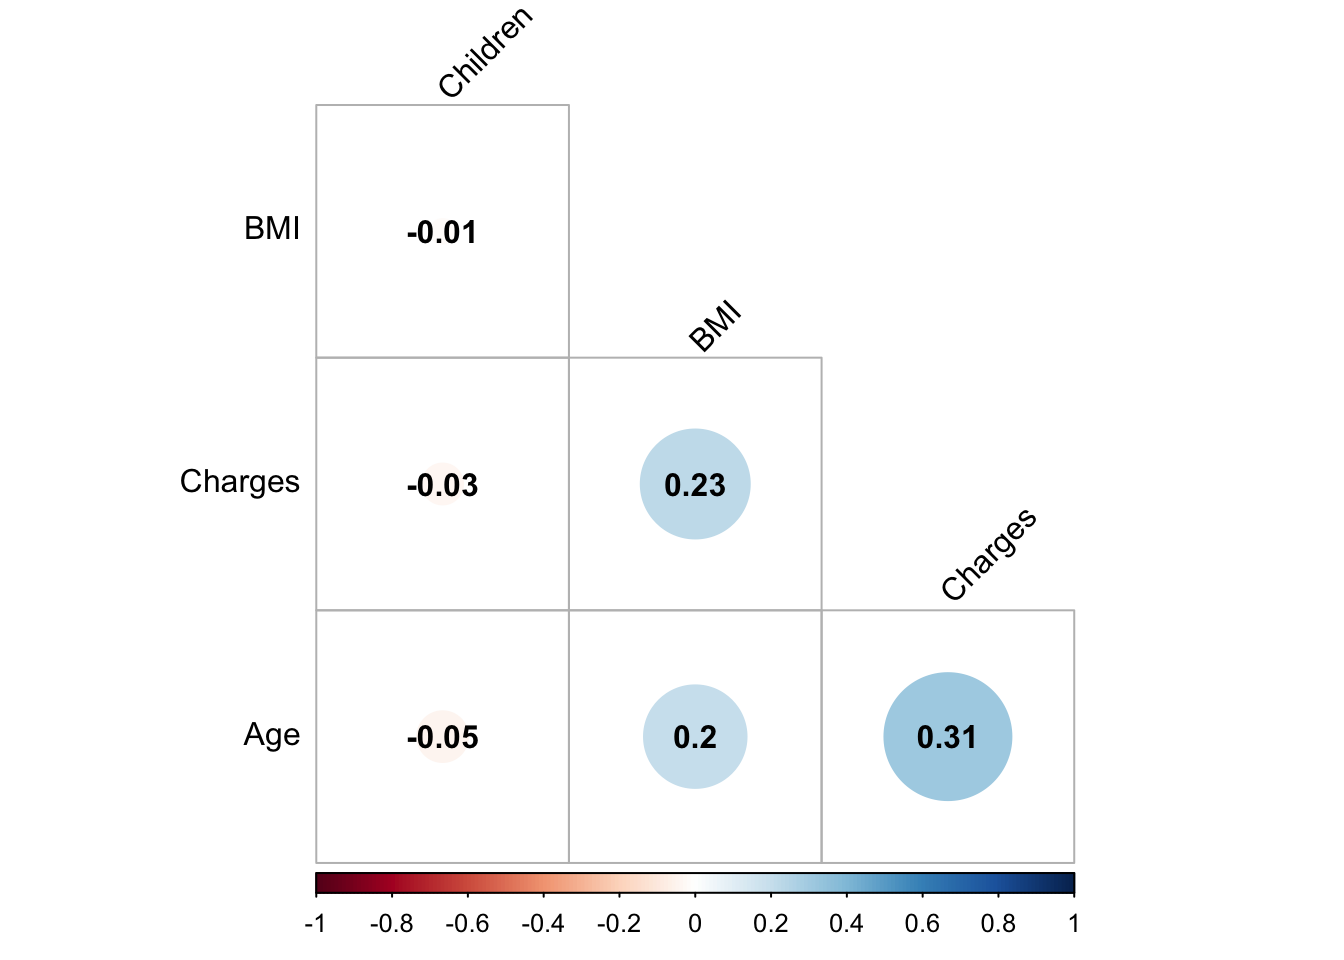
\includegraphics{CodingAssignment1_files/figure-latex/q2-1.pdf}

\begin{verbatim}
## [1] 0.2246895
\end{verbatim}

\includegraphics{CodingAssignment1_files/figure-latex/q2-2.pdf}

\begin{verbatim}
## [1] -0.04641818
\end{verbatim}

\includegraphics{CodingAssignment1_files/figure-latex/q2-3.pdf}

\begin{verbatim}
## [1] 0.2192622
\end{verbatim}

\includegraphics{CodingAssignment1_files/figure-latex/q2-4.pdf}

\begin{verbatim}
## [1] -0.01766343
\end{verbatim}

\includegraphics{CodingAssignment1_files/figure-latex/q2-5.pdf}

\begin{verbatim}
## [1] -0.04178928
\end{verbatim}

\includegraphics{CodingAssignment1_files/figure-latex/q2-6.pdf}

\hypertarget{question-3}{%
\section{Question 3}\label{question-3}}

Generate a regression equation in the following form:

\[Charges = \beta_{0}+\beta_{1}*Age+\beta_{2}*BMI+\beta_{3}*Children\]

\begin{Shaded}
\begin{Highlighting}[]
\NormalTok{ts\_model }\OtherTok{\textless{}{-}} \FunctionTok{lm}\NormalTok{(Charges }\SpecialCharTok{\textasciitilde{}}\NormalTok{ Age }\SpecialCharTok{+}\NormalTok{ BMI }\SpecialCharTok{+}\NormalTok{ Children, }\AttributeTok{data =}\NormalTok{ Health1)}
\FunctionTok{summary}\NormalTok{(ts\_model)}
\end{Highlighting}
\end{Shaded}

\begin{verbatim}
## 
## Call:
## lm(formula = Charges ~ Age + BMI + Children, data = Health1)
## 
## Residuals:
##    Min     1Q Median     3Q    Max 
## -11234  -6071  -4791   2692  28251 
## 
## Coefficients:
##             Estimate Std. Error t value Pr(>|t|)  
## (Intercept)  -5840.7     9105.8  -0.641   0.5244  
## Age            236.8      125.9   1.882   0.0662 .
## BMI            300.0      256.9   1.168   0.2488  
## Children      -311.7     1334.4  -0.234   0.8163  
## ---
## Signif. codes:  0 '***' 0.001 '**' 0.01 '*' 0.05 '.' 0.1 ' ' 1
## 
## Residual standard error: 11030 on 46 degrees of freedom
## Multiple R-squared:   0.12,  Adjusted R-squared:  0.06262 
## F-statistic: 2.091 on 3 and 46 DF,  p-value: 0.1144
\end{verbatim}

Based on the data provided, the regression equation is as follows:

Charges = -5841 + 237Age + 300BMI - 312Children

\hypertarget{question-4}{%
\section{Question 4}\label{question-4}}

An eager insurance representative comes back with a potential client.
The client is 40, their BMI is 30, and they have one dependent. Using
the regression equation above, predict the amount of medical expenses
associated with this policy. (Provide a 95\% confidence interval as
well)

\begin{Shaded}
\begin{Highlighting}[]
\NormalTok{newPrediction }\OtherTok{\textless{}{-}} \FunctionTok{data.frame}\NormalTok{(}\AttributeTok{Age =} \DecValTok{40}\NormalTok{ , }\AttributeTok{BMI =} \DecValTok{30}\NormalTok{ , }\AttributeTok{Children =} \DecValTok{1}\NormalTok{)}
\FunctionTok{predict}\NormalTok{(ts\_model,}
\AttributeTok{newdata =}\NormalTok{ newPrediction,}
\AttributeTok{interval =} \StringTok{"confidence"}\NormalTok{,}
\AttributeTok{level =}\NormalTok{ .}\DecValTok{95}\NormalTok{)}
\end{Highlighting}
\end{Shaded}

\begin{verbatim}
##        fit      lwr      upr
## 1 12321.89 8913.548 15730.23
\end{verbatim}

The result indicates that the insurance representative can expect the
value in medical expenses to be about 12,321.89 and that they can be 95
percent confident that the true value lies somewhere between 8,913,55
and 15,730.23.

\end{document}
